%!TEX root = ../../thesis.tex


\graphicspath{{Chapters/background/figures/}}

\chapter{Background} \label{chapter:background}
\section{Introduction}
In this chapter the basic foundation of computer vision models will be presented, starting
from the basics of neural networks in Section~\ref{sect:nn_basics}. From there,
the general techniques used to train neural networks will be covered in
Sections~\ref{sect:nn_train_start} through~\ref{sect:nn_train_end}, along with more
specific tools that can be used to extract higher performance. With the foundations of simple networks and
network training laid, Sections~\ref{sect:nn_advanced_start} through~\ref{sect:nn_advanced_end} discuss the more complex,
computer vision-specific operations, as well as how they combine to form convolutional neural networks.
Additionally, the benchmark datasets used commonly in computer vision research are introduced in
Section~\ref{sect:data_policies}. Finally, Section~\ref{sect:hardware} describes
the software and hardware necessary to work with these kinds of neural networks.
This all serves to provide the conceptual background required to discuss the
more specific literature that appears in the subsequent chapter.

\section{Neural Networks} \label{sect:nn_basics}
\subsection{Neuron}
The absolute foundation of neural networks is the artificial neuron. In the simplest case, an artificial neuron takes
a vector of inputs $[x_0, x_1, \dots, x_n]$ and computes:
\begin{align}
	y = f \left(\sum_{i=0}^{n} \theta_{i} x_i \right) \label{eq:ffw_layer}
\end{align}
\noindent where $\vec{\theta}$ is a vector of size $n$ that controls the weighting of each input to the neuron and $f$ is referred
to as the \textit{activation function}~\citep{anthony2001}. Also common is the addition of a bias $b$, which allows the neuron to
represent a y-intercept within the internal sum:
\begin{align}
	y = f \left(b + \sum_{i=0}^{n} \theta_{i} x_i \right)
\end{align}

This activation function $f$ varies depending on the desired properties of the neuron, but is typically a nonlinear function
that maps $\mathbb{R}\rightarrow\mathbb{R}$ or some subset of $\mathbb{R}$  (more on activation functions in Section~\ref{sect:nonlinearities}). The real magic of the artificial neuron is
the weight vector $\vec{\theta}$ and the bias $b$, the values of which can adapt or `learn' to better serve the needs of the neuron. These weights
are referred to as the \textit{learnable parameters} of the neuron, and the process of learning these weights is referred to as
\textit{training} which will be explored in more depth shortly. The more inputs to a neuron, the more learnable parameters it needs to have,
which comes at the expense of computational cost and training complexity.

\subsection{Feedforward Networks} \label{sect:ffw}
If $m$ neurons are stacked in parallel such that all receive the same $n$ inputs $[x_0, x_1, \dots, x_n]$, their
joint output can be expressed as:
\begin{align}
	\vec{y} &= f(\mathbf{\theta}\vec{x} + \vec{b}) \\
	\begin{pmatrix}
		y_{1} \\
		y_{2} \\
		\dots \\
		y_{m}
	\end{pmatrix} &= f \left( \begin{pmatrix}
		\theta_{11} & \theta_{12} & \dots & \theta_{1n} \\
		\theta_{21} & \theta_{22} & \dots & \theta_{2n} \\
		\dots    & \dots    & \dots & \dots \\
		\theta_{m1} & \theta_{m2} & \dots & \theta_{mn}
	\end{pmatrix}\begin{pmatrix}
		x_{1} \\
		x_{2} \\
		\dots \\
		x_{n}
	\end{pmatrix} + \begin{pmatrix}
		b_{1} \\
		b_{2} \\
		\dots \\
		b_{m}
	\end{pmatrix}\right),
\end{align}

\noindent where the activation function $f$ is applied elementwise to the vector.
This formulation is called a fully-connected layer, which for $n$ inputs and $m$ neurons has an $m$x$n$ matrix
of learnable weights and $m$ learnable biases. By composing these layers together into larger \textit{feedforward networks},
such that the outputs of one layer are sent to the inputs of subsequent layers, the relatively simple
function approximations of a single neuron can be built into much more complex functions. For such a stacking of $L$ layers, the network
output is:
\begin{align*}
	\vec{y_0}&= f_0(\mathbf{\theta}_0 \vec{x} + \vec{b_0}) \\
	\vec{y_1} &= f_1(\mathbf{\theta}_1\vec{y_0} + \vec{b_1}) \\
	\dots \\
	\vec{y_L} &= f_L(\mathbf{\theta}_L\vec{y_{L-1}} + \vec{b_L})
\end{align*}

In fact, with enough neurons per layer, these \textit{feedforward networks} become Universal
Approximators~\citep{stinchcombe1989}, that is, capable of approximating any arbitrary function that maps $\mathbb{R}^{n_{in}}$ to
$\mathbb{R}^{n_{out}}$, where $n_{in}$ is the number of network inputs and $n_{out}$ is the number of network outputs. However, the larger the network, the more computational power and time
necessary to calculate the network output $\vec{y}$ for some input $\vec{x}$.
Additionally, the number of learnable parameters is $\sum_{l=1}^L (m_l * m_{l-1} + m_l)$, where $m_l$
is the number of neurons in layer $l$ and $m_0$ is the number of network inputs $n_{in}$.

With this, the simplest forms of neural networks have been outlined. Before discussing any more advanced network
design concepts, it is first necessary to explore how these networks are actually trained.

\section{Supervised Learning} \label{sect:nn_train_start}
As shown in Section~\ref{sect:ffw}, neural networks are essentially a function $f(x, \mathbf{\theta})$ that,
given some input $x$ and its learnable parameters $\mathbf{\theta}$, approximates some desired function $F$.
The question is, how should $\mathbf{\theta}$ be learned such that the desired function is accurately modeled? In situations where
samples of the mapping are available, that is, both a set of inputs $\mathbf{X}$ and corresponding \textit{labels} $\mathbf{Y}$ such that:
\begin{align}
	F(x) = y \quad \forall x,y \in \mathbf{X}, \mathbf{Y}
\end{align}
\textit{supervised learning} can be performed to learn the
parameters. This is the process of learning some $\mathbf{\theta}$ such that $f(x, \mathbf{\theta}) \approx y$ for all $x,y \in \mathbf{X}, \mathbf{Y}$,
performed by minimizing a \textit{loss function}.

\subsection{Loss Functions}
Loss functions are functions that measure the distance between the ground-truth label $y$ and the model output
$f(x, \mathbf{\theta})$, the latter quantity named the \textit{prediction} of the model.
Often, these are measured over the entire set of input values $\mathbf{X}$, producing a single value that summarizes the
general distance between all of the ground truth values and all of the predictions. For models that are attempting
to learn a regression, a mapping from some input $x\in \mathbf{X}$ to some arbitrary number or numbers, common loss functions are
based around common distance metrics such as mean square error:
\begin{align}
	L_{mse}(\mathbf{Y}, \;f\left(\mathbf{X}, \mathbf{\theta} \right)) = \frac{1}{|\mathbf{X}|} \sum_{x,y \in \mathbf{X}, \mathbf{Y}} \left(y - f(x, \mathbf{\theta})\right)^2
\end{align}

In classification tasks, where the desired label is some integer or integers that represents a discrete
classification of the input, the model output is often formatted as a probability vector $\vec{y}$, where $y_i$ represents
the model's belief that the input belongs to the $i$th class. In this instance, the goal is to maximize $p(y | x, \mathbf{\theta})$,
which can be accomplished by performing maximum likelihood estimation. This means a logical choice for loss function is \textit{negative log
likelihood}~\citep{goodfellow2016}:
\begin{align}
	L_{nll}(\mathbf{Y}, \;f\left(\mathbf{X}, \mathbf{\theta} \right))  = - \frac{1}{|\mathbf{X}|} \sum_{x,y \in \mathbf{X}, \mathbf{Y}} \log p(y | x, \mathbf{\theta} )
\end{align}

\noindent Negative log likelihood is often referred to in literature as \textit{cross-entropy loss}, and this convention is used
within this thesis as well.

Notice in both of these cases $L=0$ represents the optimal condition where the predictions exactly match the ground truth
labels. As such, the training process is commonly represented as the following optimization:
\begin{align}
	 \text{argmin}_{\mathbf{\theta}} L\left(\mathbf{Y}, \;f\left(\mathbf{X}, \mathbf{\theta} \right)\right)
\end{align}
\noindent Thus, the loss function should map $\mathbf{Y}$ and $f(\mathbf{X}, \mathbf{\theta} )$ into $[0, \infty)$, where 0 marks the optimal result.
While the above are just examples of some common loss functions for two common types of network, any function $L$ that maps
the desired ground truth outputs and model predictions into $[0, \infty)$ could in theory be used as a loss function.


\section{Stochastic Gradient Descent} \label{sect:sgd}
The problem of optimizing the parameters of a neural net is notoriously tricky. Neural nets can have upwards of a
billion parameters in extreme cases~\citep{huang2018}, meaning that optimizing said parameters to minimize error is a
multi-billion dimensional optimization problem, which is mathematically intractable. Additionally, networks
of any meaningful scale are expensive in time and computation to evaluate, which limits the number of samples
that may be drawn from the parameter space. To approach this problem,
stochastic sampling methods can be used. The most prominent technique for such optimization is \textit{gradient descent}~\citep{goodfellow2016}.
Gradient descent is used to minimize loss functions, and does so through iterative minimization. This is done by stepping
the model parameters $\mathbf{\theta}$ in the direction that most decreases $\mathit{L}$:
 \begin{align}
 	\label{eq:SGD} \Delta \mathbf{\theta}_t = - \eta \nabla \mathit{L}(\mathbf{\theta})
 \end{align}
 where $\eta$ is referred to as learning rate. To translate this gradient into meaningful updates of each parameter, the
partial derivative of the loss with respect to each parameter is computed by traversing the model backwards. This
allows the use of the chain-rule to quickly compute these partial derivatives, meaning that each parameter need
only be aware of the gradient of its output. This process of propagating the errors back up the model is referred
to as \textit{backpropagation}, and is the mathematics at the very heart of network training.

During each gradient update step performed in gradient descent, $\mathit{L}(\mathbf{\theta})$ can be computed
in a variety of different ways and contexts. If the desire is to minimize loss over the entirety of the training dataset at once,
the loss can be taken as the average of the loss
of each datapoint in the training data. The step that the model will then take in gradient descent would be one that
minimizes the average loss over the entire data. However, this would be tremendously expensive to compute in terms
of memory; the gradients of each parameter with respect to each input would need to be stored. Considering a reasonable
training dataset for a neural network is on the order of tens of thousands of data points at the very least, and model parameters
are usually on the order of hundreds of thousands if not millions, this would be prohibitively expensive. On the other
hand, gradient updates could be performed for each datapoint, computing $\mathit{L}(\mathbf{\theta})$ as the loss for
each specific point. The disadvantage with this single-datapoint approach is that many neural network
computational libraries can make use of massive parallelization when processing multiple inputs, and backpropagating
inputs one at a time through the model is the least efficient use
of that capability. Additionally, tuning the entirety of the model parameters to suit a single input is likely heavy-handed as
specifically tailoring the model to a single input will likely be detrimental to the performance over all the rest. As a compromise,
$\mathit{L}(\mathbf{\theta})$ can be computed from a small batch of the input dataset, then the model updated to minimize loss over
that specific batch. This means that each gradient update will be performed with respect to a variety of inputs, while still being
able to take advantage of parallelization. This process is referred to as \textit{minibatch stochastic gradient descent}~\citep{goodfellow2016}.
However, in the literature it is common to see minibatch SGD referred to as simply stochastic gradient descent, and this
thesis will use the same convention.

This process can be thought of as navigating some multi-dimensional parameter landscape, with the position
in this landscape given by the current coordinates $\mathbf{\theta}$, and the `height' at that position given by
$L(\mathbf{\theta})$. To find the lowest point in that landscape, a step of size $\eta$ in
the direction  $-\nabla L(\mathbf{\theta})$, that is, opposite from the direction of steepest gradient, could potentially
move downwards and thus decrease the loss. Of course, the gradient at the current position might radically change
over the span of the step of size $\eta$, thus the next step through this unseen territory might end up worsening the loss.
Smaller values of  $\eta$ minimize this risk, as they minimize the unknown space stepped over, but result in needing
to take more steps (and thus increasing the number of expensive samples to perform). Additionally, smaller values
of $\eta$ increase the likelihood of getting stuck in local minima; if the step is not big enough to step up and out
of a local minima then the model might end up `circling the drain' forever. Larger values of $\eta$ can more quickly cover
a broader expanse of the parameter landscape and step out of small local minima. However, this also means that each
step travels through more unseen terrain, which could potentially step through areas of significant gradient change and into
significantly worse positions. The process of conducting an effective stochastic gradient descent is thus balancing and
moderating this $\eta$ to get the best of both the large and small $\eta$ regimes. A common way of achieving this is
through learning rate annealing, wherein the descent process is started with a large $\eta$ value, such as to explore a
large swath of the loss landscape, but this learning rate is then slowly lowered over the course of training such as to introduce
finer and finer tuning steps as the model settles into its final minimum~\citep{goodfellow2016}.

Stochastic gradient descent, by the very nature of being a stochastic algorithm working on a tremendously complex loss
landscape, is sensitive to initial conditions, algorithmic parameters, and idiosyncrasies in the loss geometry.
There is a variety of techniques that can be applied to mitigate these factors and improve the stability and performance
of SGD; chiefly, momentum and weight decay.

 \subsection{Momentum}
 Momentum appends a term into the SGD function:
 \begin{align}
 \Delta \mathbf{\theta}_t = - \eta \nabla \mathit{L}(\mathbf{\theta}_t) +  p \Delta \mathbf{\theta}_{t-1}
 \end{align}
This term adds some fraction $p$ of the previous step into the current step, literally adding a momentum
to the movements through the parameter landscape. This speeds up the movement on extended descents, as well as allows
for rolling up and out of local minima at smaller learning rates than would be possible otherwise.

\begin{figure}[ht!]
	\centering
	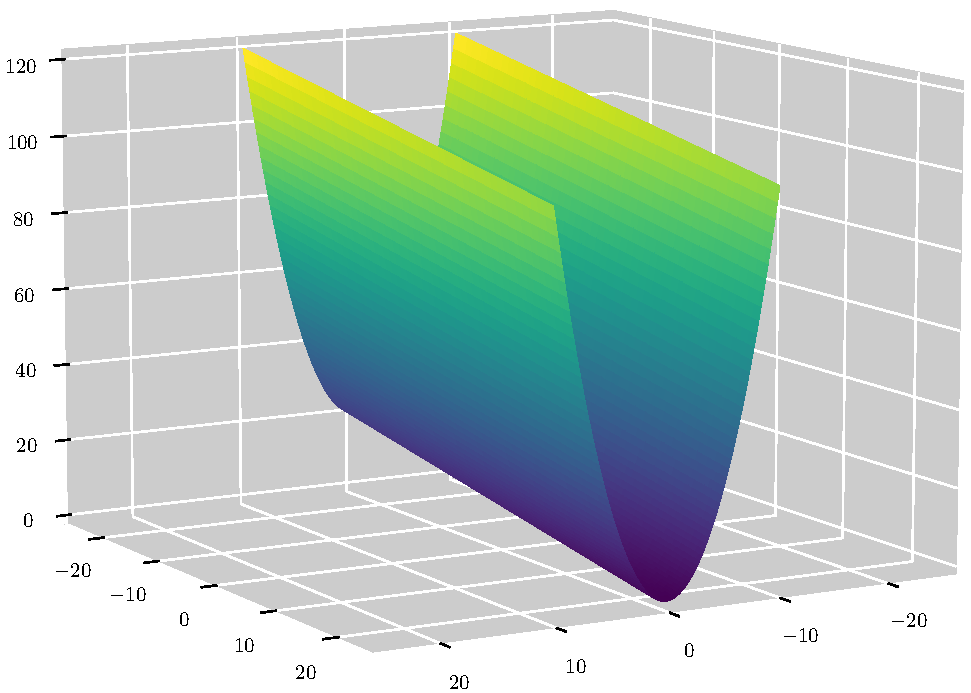
\includegraphics[width=.5\textwidth]{momentum/long_and_narrow}
	\caption[Qian's long and narrow valley example]{A long and narrow valley as described by~\cite{qian1999}.}
	\label{fig:long_and_narrow}
\end{figure}

In one of the first
exploratory papers of the concept,~\cite{qian1999} describes a particular geometric case of a ``long and
narrow valley,'' (see Figure~\ref{fig:long_and_narrow}) which slopes gradually down along the long axis of the valley. Along the floor of the valley, the
gradient points along the short axis of the valley, that is, up the valley walls, as this is the direction of greatest slope.
This means a standard SGD algorithm will oscillate roughly in line with the short axis of the valley,
slowly traversing down the sloping long axis. The component of the loss update along the long axis will remain roughly
constant throughout the process, always pointing slightly downward along the long axis. The short axis component will
invert at each step, as the algorithm steps up and returns down each wall, meaning it will zig-zag across the walls of the valley while
only making incremental progress downwards. If a momentum term is added, some fraction of the last step persists into the current
step, therefore dampening any oscillating motion between steps while magnifying consistent motion. Figure~\ref{fig:momentum}
shows the difference in descent paths between SGD with and without momentum.

\begin{figure}[ht!]
	\centering
	\begin{subfigure}{.45\textwidth}
		\centering
		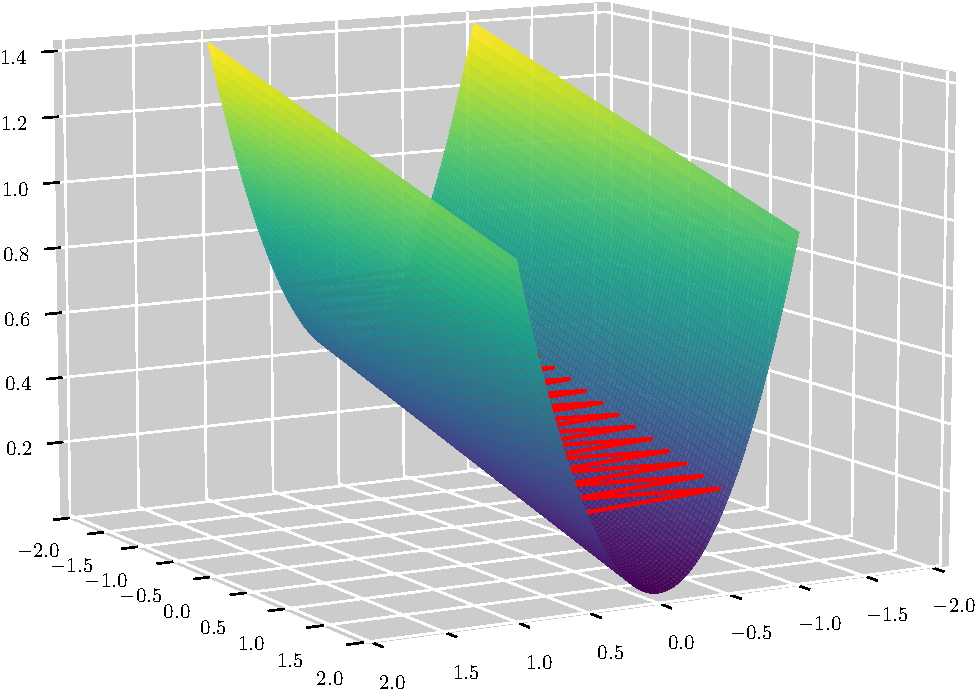
\includegraphics[width=\textwidth]{momentum/none-crop}
	\end{subfigure}
	\begin{subfigure}{.45\textwidth}
		\centering
		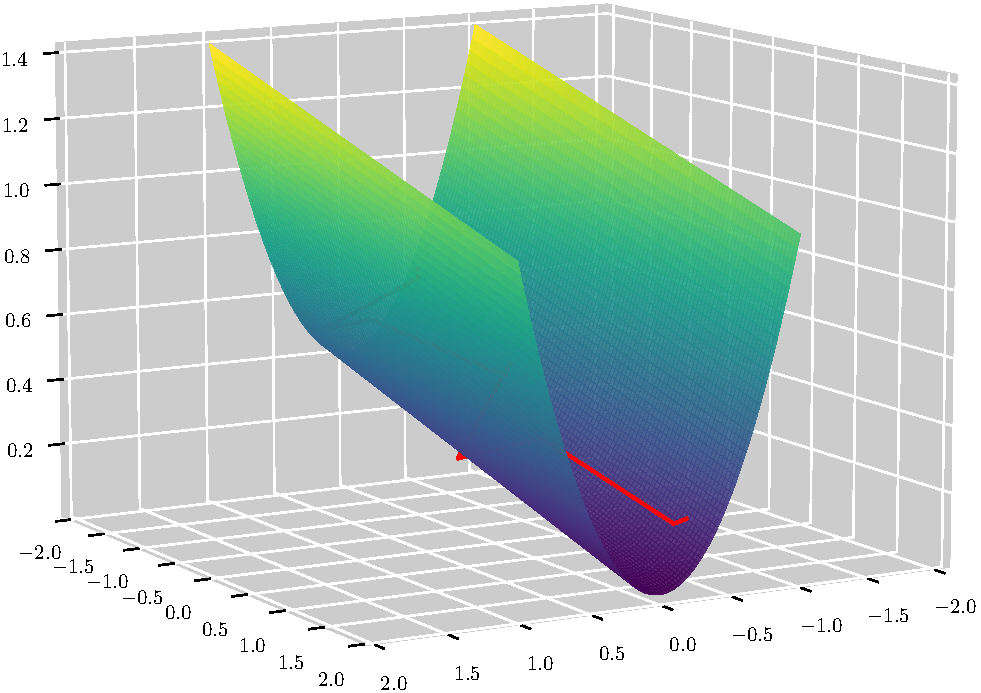
\includegraphics[width=\textwidth]{momentum/p9crop}
	\end{subfigure}
	\caption[Comparison of SGD with and without momentum]{Starting at the point $x=0.5, y=-2$ these figures show the path taken by SGD as it attempts to descend to $f(x,y)=0$.
	At left, SGD is performed without momentum, whereas the right uses a momentum value of $0.9$.}
	\label{fig:momentum}
\end{figure}

This accelerating factor and oscillatory
dampening in strange geometries is exactly the benefit of momentum, and since loss landscapes often feature incredibly
complex geometries, momentum is a crucial tool to best perform efficient gradient descent.

 \subsection{Weight Decay}
Weight decay~\citep{krogh1992} adds a L2 regularization to the loss function:

\begin{align}
	\mathit{L}(\mathbf{\theta}) = \sum_i (\mathit{L}(\mathbf{\theta_i})) + \frac{1}{2} \lambda \sum_{i} \mathbf{\theta}_{i}^{2}
 \end{align}
thus penalizing large values of $\vec{\theta}$ by some factor $\lambda$. The effect of this is to both reduce the
number of possible `good' places in the loss landscape to traverse to, as ones further from the origin will be
more heavily penalized, while also preventing model overfitting to some degree; the model cannot travel to extreme
lengths to contort itself to the training data, instead being obliged to focus on more general solutions in the more localized
loss landscape.

\subsection{Other Optimizers}
Stochastic gradient descent is just one of many such optimizers that perform efficient searches of the loss landscape
to find optimal model parameter values. Another highly popular choice is the Adam algorithm~\citep{kingma2015}, which uses
running means and variances of the loss gradient to inform the direction and magnitudes of weight updates. However,
the performance of various optimizer algorithms is highly dependent on both their application and choice of specific
tuning parameters, which means that the most crucial differentiating factor in their performances is often just
how familiar the user is with the algorithm's particular nuances~\citep{goodfellow2016}. Much of the literature that most
directly pertains to this thesis makes heavy use of SGD over any other algorithm, and as such is the exclusive choice
for optimizers in this work. For more information about other optimizers, see~\cite{goodfellow2016}.

\section{Neural Network Strategies} \label{sect:nn_train_end}
\subsection{Validating Model Fitting}
While stochastic gradient descent and backpropagation are effective tools to ensure that neural models learn some $\mathbf{\theta}$ such
that $f(\mathbf{X}, \mathbf{\theta})\approx \mathbf{Y}$, there are a couple of pitfalls that this learning process can fall into. First is
\textit{underfitting}, where the model is unable to accurately approximate the desired function and its predictions;
the model simply does not know the material well enough to succeed. This can be caused by a number of factors, usually
insufficient training time or insufficient model
complexity. The former occurs when the model has not seen enough samples of $x, y$ pairs (where $x \in X$, $y \in \vec{y}$)
to learn the nuances of the desired function. An easy analogy for this circumstance is not studying enough for an
exam; the model has simply not spent enough time reviewing the exam material to perform well. The latter occurs when
the model's $\mathbf{\theta}$ is not large enough to model the desired function; remember the conclusion of the Universal Approximation
Theorem from~\ref{sect:ffw} only applies to sufficiently large models. An analogy that can be drawn is trying to fit a polynomial regression
$y = \sum_{i=0}^{n} \beta_i x^i$. If there are $[x, y]$ samples $[0, 0],\;[1, 1],\;[2, 4],\;[3, 9],\;[4, 16]$, it is clear that
the function being modeled is $x^2$. However, if the polynomial regression model is constrained to $n=1$, no amount
of fitting will adequately model the desired function. This is exemplary of the second main cause of underfitting, insufficient
model complexity.

On the other hand is \textit{overfitting}. This is when the model has managed to essentially `memorize'
the training data, simply memorizing that $f(x_1, \mathbf{\theta})$ and $f(x_2, \mathbf{\theta})$ should equal $y_1$ and $y_2$ without actually learning
\textit{why}. This happens due to two main causes; insufficient amounts of training data or too much model complexity. The
earlier polynomial regression example can easily demonstrate the former cause. In this case, if there are only three samples
$[-1, 1],\;[0, 0],\;[1, 1]$, there are an infinite range of polynomials that would fit this data perfectly;
$y=x^n$ for any even $n$, for example. Despite all of these functions having perfect accuracy over the sample data,
it cannot be definitively stated that they have modeled the desired function; there are simply not enough data samples to have
any inkling as to the true function. The latter case occurs when the model is large enough that it has enough
flexibility that it can essentially just act as a lookup table; input 1 should return output 1, input 2 should return output 2,
etc.

With these two potential pitfalls, it is crucial to understand how to diagnose when a model has fallen into one. The answer is through the
use of data splits. In the simplest form, data samples are divided into two sets, a \textit{training set} and
a \textit{test set}. Only data from this training split is used when training the model. Two metrics can then
determine how the model is faring; training set and test set performance. Since the exact metric to measure `performance'
can vary depending on the particular task at hand, good and bad performance will be referred to qualitatively
rather than quantitatively for these examples. Training set performance can reveal how well the model is able to
emulate the training samples, and determine whether it has sufficient flexibility to model the function. If the training set
performance is satisfactory, it should at be least capable of the desired modelling. Then,
the test set performance can be investigated to get a measure of how well the model fares on new data from the same distribution. This
provides insight on how much of the model's training performance is learning the desired function or is simply memorization.
Good test set performance means the model is accurately predicting the correct outputs for new inputs, despite having never
seen these datapoints before. This implies that it is in fact modelling the desired function (or at least one that produces
the desired outputs for both the training and test inputs). Good train performance but poor test performance implies that
the model has simply memorized the train datapoints but has no knowledge of the true underlying function to use on novel datapoints.
The possible permutations are listed in Table~\ref{tab:traintestfitting}:
\begin{table}[h]
	\begin{center}
	\begin{tabular}{c|cc}
		 						& Good Test Performance & Poor Test Performance	\\ \hline
		 Good Train Performance & The model is well-fit & Overfit 		\\
		 Poor Train Performance & 		Rare			& Underfit		\\
	\end{tabular}
	\end{center}
	\caption[Indicators of over and underfitting]{The various permutations of the two metrics. The lower left state (poor train, good test performance) is unusual,
		and perhaps indicates that the train and test sets come from different data distributions and are thus not
		particularly useful for diagnosing model fit.}
	\label{tab:traintestfitting}
\end{table}

With these tools it is now possible to identify when a model is moving towards one of these training pitfalls; however,
what can be done to avoid them? This question has produced an immensely rich vein of research,
particularly in the early 2010s as model size began to skyrocket and overfitting issues became more widespread. In particular, strategies
within both data preprocessing and the training policies are particularly useful in avoiding both issues.

\subsection{Data Preprocessing}
Data preprocessing refers to everything done to the data to before passing it into the model. The most common processing
done to input data is to standardize and normalize it for the model. Data standardization refers to the process of
ensuring each input tensor to the model is of the same shape, that is, having equal size along each of the dimensions.
For the types of models discussed here, they are either only capable of operating over fixed size inputs or perform
better when that is the case. In the case of image data, typically dimensions to which most of the inputs
roughly conform are picked, and then input images are either scaled or cropped to ensure that they all have uniform
size~\citep{kriv2012}. Normalization on the other hand is simply ensuring that the values of each of the input datapoints
come from roughly the same distribution. Typically, each input to a model is normalized by subtracting the dataset mean $\mu_X$
and scaling by the dataset standard deviation $\sigma_X$:
\begin{align}
	x' = \frac{x - \mu_X}{\sigma_X} \quad \forall x \in X.
\end{align}

This ensures that the input dataset as a whole has a mean of 0 and a standard deviation of 1. As seen in
Figure~\ref{fig:nonlins}, most common neural network nonlinearities are most interesting between $[-1, 1]$. Significantly
outside these bounds, the nonlinearities are all mostly linear, defeating the purpose of using the nonlinearity in the first
place. Normalizing the input data ensures that it lies in this interesting region, thus maximizing the power that the
network can provide.

Another data strategy that can be performed to maximize the value of the input dataset is \textit{augmentation}. This is the
process of transforming and modifying the input data such as to increase the total number of datapoints that are available.
Typically, this involves looking for a set of transformations $T$ of the input data that are
\textit{label invariant}, i.e., do not modify the output labels:
\begin{align}
	f(x) = f(t(x)) = y \quad \forall t \in T.
\end{align}

\noindent These sets of transformations vary on a per-dataset, per-task basis, as the definition of label-invariance
varies depending on the type of input data and the exact mechanism of labelling. Figure~\ref{fig:image_transformations}
provides an example of this concept. This is particularly common in image data, with augmentations like horizontal
or vertical flipping, rotations, random croppings, and color jittering used fairly frequently. The power of augmentations
is that for even the simplest transformations like flipping, the amount of input data is doubled. This can be very helpful
in scenarios with small datasets which can run into overfitting issues, where the larger augmented dataset can make
it harder for the model to memorize the inputs.

\begin{figure}[ht!]
	\centering
	Task: Object Classification \\ \vspace{1em}
	\begin{subfigure}{.4\textwidth}
		\centering
		\scalebox{-1}[1]{
\includegraphics[width=.5\textwidth]{data/fiesta}}
		\caption{$f(x) = \texttt{car}$}
	\end{subfigure}
	\begin{subfigure}{.4\textwidth}
		\centering
		
\includegraphics[width=.5\textwidth]{data/fiesta}
		\caption{$f(t(x)) = \texttt{car}$}
	\end{subfigure} \vspace{1em} \\  \hrule \vspace{1em}
	Task: Letter Classification \\ \vspace{1em}
	\begin{subfigure}{.4\textwidth}
		\centering
		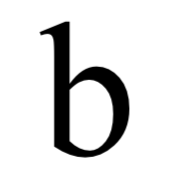
\includegraphics[width=.5\textwidth]{data/b}
		\caption{$f(x) = \texttt{b}$}
	\end{subfigure}
	\begin{subfigure}{.4\textwidth}
		\centering
		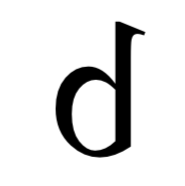
\includegraphics[width=.5\textwidth]{data/b_flip}
		\caption{$f(t(x)) = \texttt{d}$}
	\end{subfigure}
\caption[Various augmentations and how they potentially permute data labels]{Horizontal flipping augmentation applied to two different image classification tasks. In the first, horizontal
flipping does not change the label of the image; a mirror image of a car is still a car. In the second, horizontal flipping
changes the label of the image from $\texttt{b}$ to $\texttt{d}$. This is an excellent example of why augmentation policies
need to be chosen on a per-dataset, per-task basis; despite both datasets being image classification tasks, this augmentation
policy is only valid for the first.}
\label{fig:image_transformations}
\end{figure}

Furthermore, augmentation can be used to describe or reinforce desirable properties
of the mapping that the network is trying to learn. For example, if it is known that the desired mapping is commutative,
an augmentation that randomly shuffles the order of values within the inputs can be applied. This will directly demonstrate
to the model that the order of values within the input does not matter to the final labelling, which forces it to also
produce a commutative mapping if it wants to be performant. In the case of image data, encouraging
translational invariance (regardless of where an object appears in a picture, it does not change the properties of said object) can be helpful. Doing this entails grabbing a random subcropping of
each image and then padding them back to the desired dimension. This will shift the contents of the image by however much
the center of the random cropping differs from the center of the original image, thus demonstrating the desired translational
invariance. Augmentation, by both increasing the amount
of data that the model is exposed to and enforcing useful strategies that the model can apply to better learn the data,
can help with both under and over-fitting.

While the previous two strategies have been mainly focused on making the tasks easier for the model to learn, data preprocessing can also be used
to apply \textit{regularization}. Regularization is essentially a limitation that is applied to constrict
the valid solutions to the problem, in such a way that the model is guided to a more suitable or better performing answer.
In terms of data preprocessing, a very common regularization that is applied particularly to image data is Cutout, introduced
by~\cite{devries2017}. Cutout simulates object occlusion, by
cutting out a square section from a random location of the input image, as demonstrated in Figure~\ref{fig:cutout}.

\begin{figure}[ht!]
	\centering
	\begin{subfigure}{.4\textwidth}
		\centering
		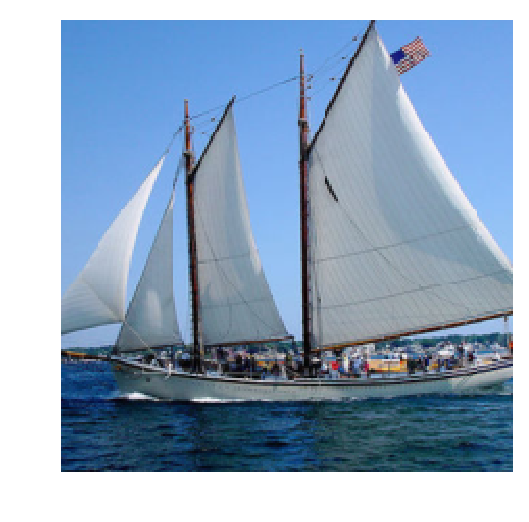
\includegraphics[width=.75\textwidth]{data/cutout_off0}
	\end{subfigure}
	\begin{subfigure}{.4\textwidth}
		\centering
		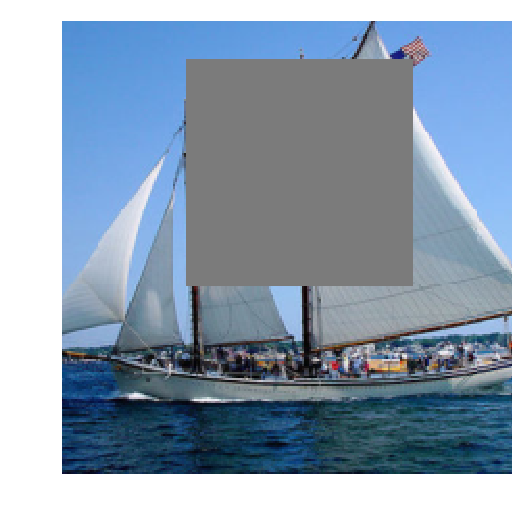
\includegraphics[width=.75\textwidth]{data/cutout_on0}
	\end{subfigure} \vspace{1em} \\  \hrule \vspace{1em}
	\begin{subfigure}{.4\textwidth}
		\centering
		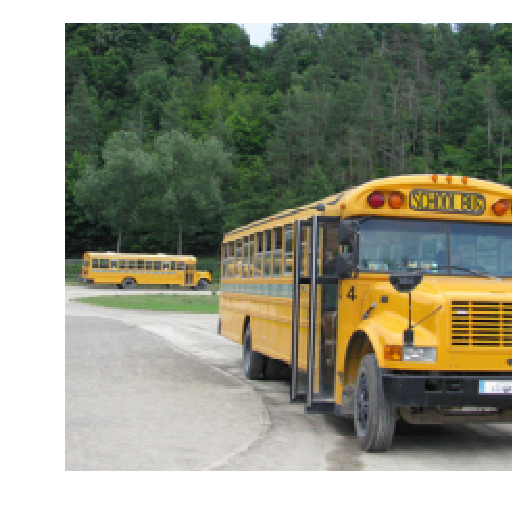
\includegraphics[width=.75\textwidth]{data/cutout_off-1419}
	\end{subfigure}
	\begin{subfigure}{.4\textwidth}
		\centering
		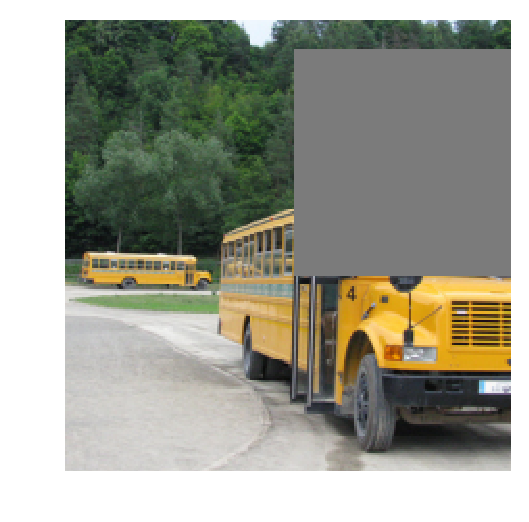
\includegraphics[width=.75\textwidth]{data/cutout_on-1419}
	\end{subfigure}
\caption[Cutout applied to different ImageNet images]{Cutout applied to different images from the ImageNet dataset. The cutout area is typically replaced with the
mean color from the dataset to avoid imbuing artificial color information into the data.}
\label{fig:cutout}
\end{figure}

Cutout is applied probabilistically to each input image, meaning that every time that image is passed through a model it may
potentially occur. If it does, the location at which it occurs will also be randomly chosen. This makes it very hard for the model
to memorize the input images, as particular locations that the model might otherwise latch on to cannot be
reliably trusted to appear in the image. For example, in the schoolbus image in Figure~\ref{fig:cutout} a model might
latch on to the light pattern and words ``SCHOOL BUS'' on the top of the bus, and use these to memorize
that this image is a school bus. However, if this section is cutout, that memorization is no longer possible and the model
is forced to look at other ways to correctly identify this image.  In this sense the model is forced to learn more about
the content and context of the images that it is processing, not just memorize the positions of key objects. The idea is that
the former method of learning is much more generalizable than the latter, and should therefore help the model avoid
overfitting.

Since the data constitutes the entirety of the model's knowledge of the problem and thus
its potential to learn, it is critical that data strategies like normalization, augmentation, and regularization are used to
ensure that the teaching material is as powerful as possible.

\subsection{Training Policies}
With the potential of the data fully-extracted (ideally), the focus shifts to how the learnings from the data
are applied to the model. The methodology of how the model is trained and the strategy therein is called the training policy.

The biggest decision when it comes to training a model is setting the parameters of the training regime itself,
called the \textit{hyperparameters} of the model. These are not in and of themselves trainable parameters of the model,
but play a crucial role in the values those parameters take on. While there are essentially infinite possible
classes of hyperparameters depending on the model's specific needs and how training is implemented, the most
ubiquitous and influential are \textit{training epochs}, \textit{learning rate}, and \textit{batch size}.
Training epochs refer to the total number of times the entirety of the training data is passed through the model.
This is necessary due to the iterative nature of gradient descent, as each step can only bring the model
slightly closer to an optima. A single step improves the model, but many steps are needed to satisfactorily traverse
the loss landscape. The choice of this is often entirely dataset and model dependent, and typically is tuned through
experimentation or grid searching. In general, large epoch numbers bring good performance at the cost of compute time,
while low epoch numbers bring the opposite, and as such finding a balance is crucial.

Learning rate is identical to the learning rate described in Section~\ref{sect:sgd}, and simply indicates the size of the
step taken by the gradient descent algorithm. Choice of learning rate is crucial for the same reasons as outlined in that
section, as it determines the level of detail to which the algorithm can navigate the loss landscape. In this sense,
overly large learning rates can cause underfitting, as the model will step over finer dips and valleys in the loss
landscape and thus only be able to find coarse minima. However, a learning rate that is too small will cause training
to take a long time, as many steps are needed to get anywhere meaningful. An effective strategy to avoid making this choice
altogether is called \textit{learning rate annealing}. This
is the process of adjusting the learning rate over the course of training, such as to get benefits from both sides of the
learning rate spectrum. Typically, such strategies start with a large learning rate, to bring the model quickly from initialization
to some decent coarse minima, and then reduce the learning rate to allow for further fine optimizations. Early strategies
were often as simple as dividing the learning rate by a constant after a fixed number of epochs. A strategy like this
however tends to complicate hyperparameter choice; now the initial learning rate, the divisor, and interval between
decisions have to be chosen. Each of these has the potential to drastically affect the final performance of the model,
so rather than removing the single high-stakes choice of learning rate, two more choices are added. An annealing strategy that
I find elegantly avoids this issue is \textit{Cosine Annealing}, introduced by~\cite{loshchilov2016}.
Here, the learning rate $\eta$ at some epoch $t$ is brought from some maximum
$\eta_{max}$ to a minimum $\eta_{min}$ over the course of $T$ epochs~\citep{TorchSite}:
\begin{align}
	\eta_t = \eta_{min} + \frac{1}{2}(\eta_{max}-\eta_{min})\left(1+ \cos \left(\frac{t}{T} \pi \right)\right)
\end{align}

\noindent This way the learning rate is gradually and smoothly swept between the upper and lower bound over the entirety
of training. Typically, $\eta_{min}$ is chosen to be 0, and $T$ is equal to the total number of training epochs of the
model. This means the only thing to choose is $\eta_{max}$, and as such cosine annealing grants the benefits of learning
rate annealing without adding any extra hyperparameter selections to the model. Again, for more information about adaptive learning rates, see~\cite{goodfellow2016}.

Finally, batch size refers to the number of datapoints that are passed simultaneously to the model during training. This
turns stochastic gradient descent into batch gradient descent: rather than adjust model parameters after each individual
training data point, model parameters are updated according to the average loss gradients of all the training points within a
specific batch. Too small a batch size can result in the model making gradient updates according to idiosyncratic
information within the batch that may not generalize well, whereas too large a batch size can cause gradient updates to be
so general as to contain little meaningful information~\citep{smith2017}. Meanwhile, small batch sizes are cheap in both
computational cost and memory allocation as less concurrent data needs to be passed through the model, but many such
batches are needed to perform a full pass over the training data. Large batches can pass over the training data faster, but are
conversely more expensive to compute. As such, a balance between the two extremes is crucial to find.

Training strategies can also aim to apply regularization to the weights of the model in some way, such as to enforce
solutions that are unlikely to be overfit. The first of these is a concept called \textit{dropout}, introduced by~\cite{srivastava2014}.
Here, a random selection of connections within the model are removed
during each forward pass, essentially sampling a random subnet of the model as shown in Figure~\ref{fig:dropout}.

\begin{figure}[ht!]
	\centering
	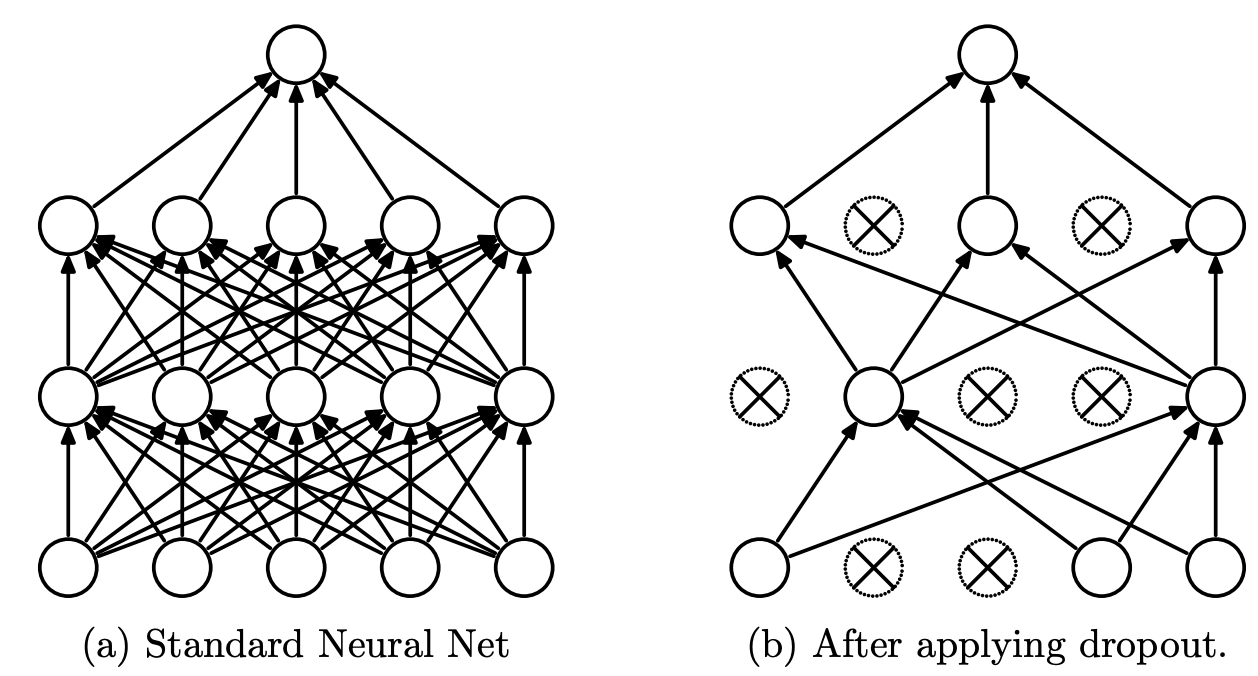
\includegraphics[width=.75\textwidth]{training/dropout}
	\caption[Dropout's effect on network connectivity]{Dropout's effect on the connectivity of a neural net, as shown in~\cite{srivastava2014}.
	The exact selection of edges to remove, and thus the exact difference between (a) and (b) changes every forward pass.}
	\label{fig:dropout}
\end{figure}

In every forward pass of the model, its exact configuration will be different, with the idea being that this reduces the
complexity of the model in an unpredictable way. This complexity is precisely the tool the model can exploit to
`memorize' the training data, by using its immense number of connections to fit to subtle details or even just noise
in the training data. When the relation between these connections cannot be guaranteed to be consistent, the model
cannot rely on pure brute force to learn the mapping. Instead,~\citeauthor{srivastava2014} note that each neuron in the model must
instead learn to be collaborative with a random sample of its fellow neurons, and cannot form the intricate
codependencies necessary to memorize the training data. As such, each neuron is forced
to robustly extract useful features without reliance on other neurons. When compared to networks trained without
dropout,~\citeauthor{srivastava2014} find that its use drastically reduces overfitting of the model, and produces significant
increases to test performance. It may seem counterintuitive that destroying a model's ability to use intricate relations
between neurons to learn highly nuanced mappings would benefit test performance, but remember that overfitting often
comes from models fitting to noise within the training data that does not exist in the test data. By preventing the
model from `cheating' in training, it is forced to learn actual insight into the task at hand, and this insight is
generalizable to new inputs. In practice, dropout is typically performed on fully connected layers in networks, with
a fixed dropout probability between $0.3$ and $0.5$ during training and $0.0$ during testing.

\begin{figure}[ht!]
	\centering
	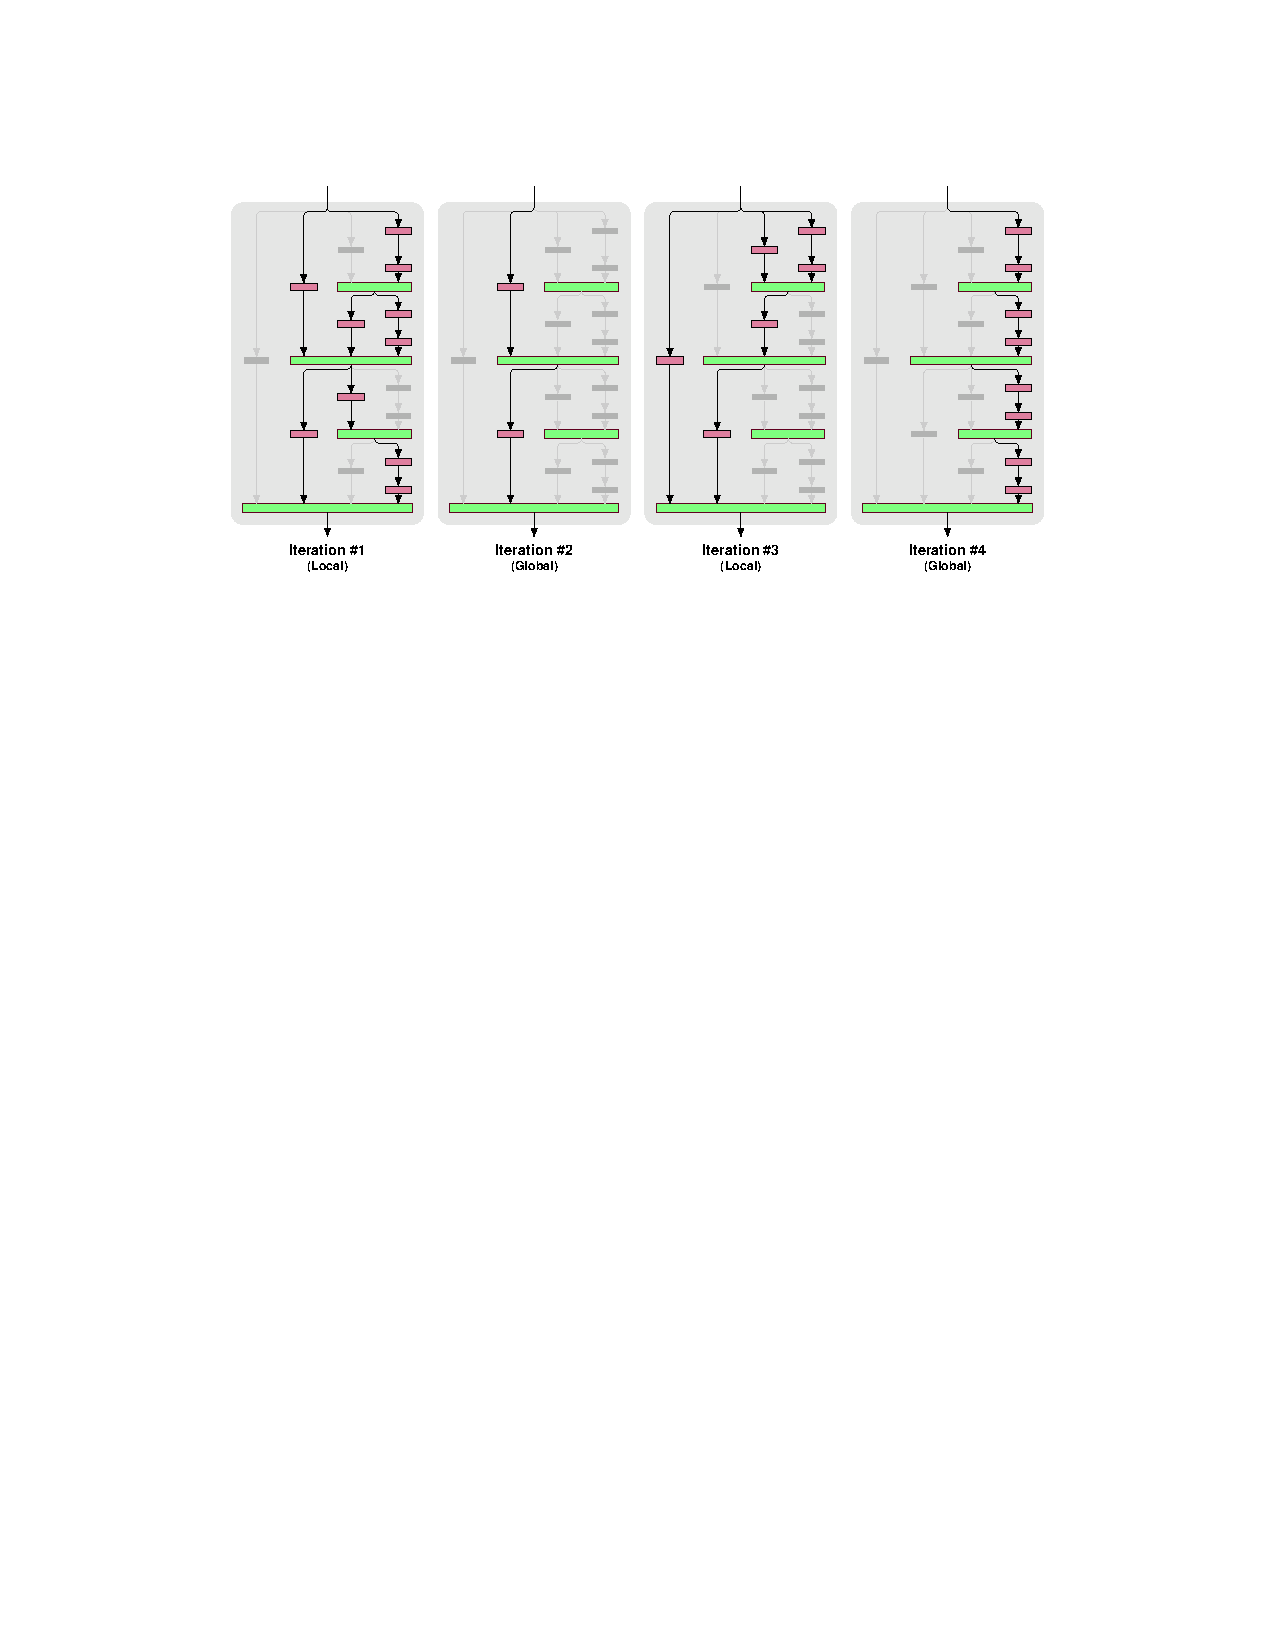
\includegraphics[width=.95\textwidth]{training/droppath}
	\caption[Local and global Drop-Path's effects on connectivity]{Local and global Drop-Path's effects on the connectivity of a neural net, as shown in~\cite{larsson2016}.}
	\label{fig:droppath}
\end{figure}

This regularization-via-removal concept can be extended to network architectures as a whole, and drop out entire pathways
through the model. This process is referred to as Drop-Path~\citep{larsson2016}, and can operate over two different scales:
local or global. Local Drop-Path looks granularly at individual layers of the network architecture, specifically at the various
inputs to any given layer. These inputs are then randomly dropped during training, while still ensuring that at least one
path always remains to the input. Global Drop-Path instead looks at each possible path from the network input to output,
and randomly samples a single one at each training step. Figure~\ref{fig:droppath} shows graphically the effects of both
local and global Drop-Path. Together, they ensure that the paths to particular layers and the
various paths through the model are all independently capable of producing good results, improving a model's strength
and robustness.


\section{Beyond Feedforward Networks} \label{sect:nn_advanced_start}
Fully-connected layers can be tremendously powerful in large numbers and can learn to approximate any
function that might be needed. However, by complementing these layers with other types of operations their
power can be greatly expanded. Furthermore, directly inserting layers that have useful mathematical properties will reduce
computational cost and time, since it bypasses the network training needed to approximate those functions organically.
In general, all such operations are formulated as tensor operations, typically performed using linear algebraic functions
which allows for fast parallel processing (see Section~\ref{sect:hardware} for more details).

\subsection{Tensor Operations}
A tensor, at least for the purposes of this work, is simply the n-dimensional generalization of vectors and matrices.
An order-1 tensor is a vector, an order-2 is a matrix, and so on, and the data that flows through deep learning models are represented in this form.

\begin{figure}[ht]
	\centering
	\begin{subfigure}{.33\textwidth}
		\centering
		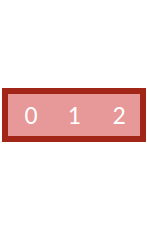
\includegraphics[height=10em]{tensors/order1}
		\caption{Order-1 tensor (vector)}
	\end{subfigure}
	\begin{subfigure}{.33\textwidth}
		\centering
		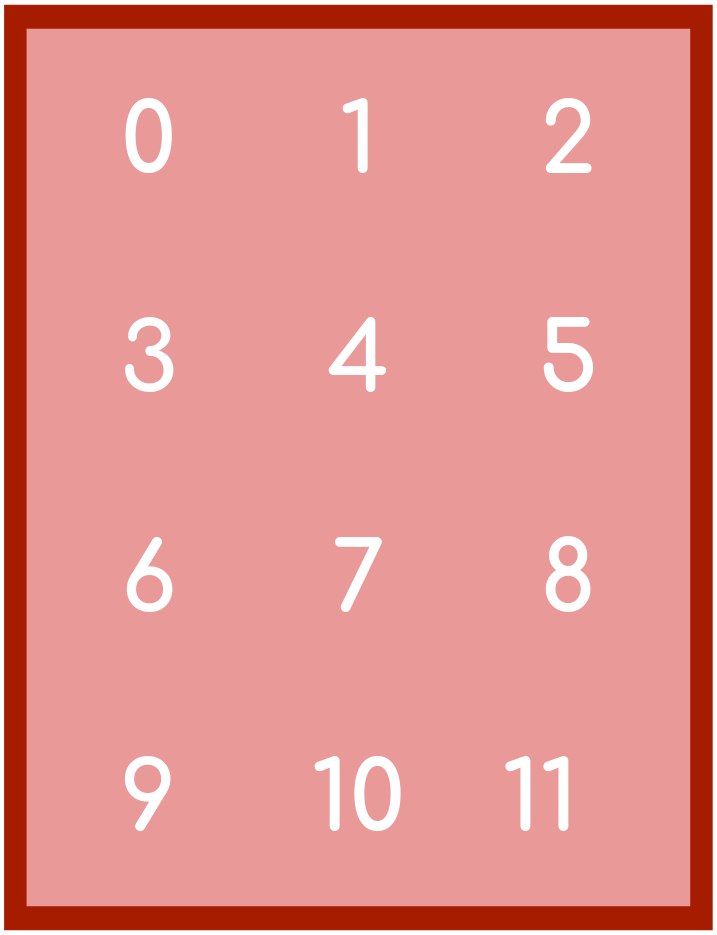
\includegraphics[height=10em]{tensors/order2}
		\caption{Order-2 tensor (matrix)}
	\end{subfigure}
	\begin{subfigure}{.3\textwidth}
		\centering
		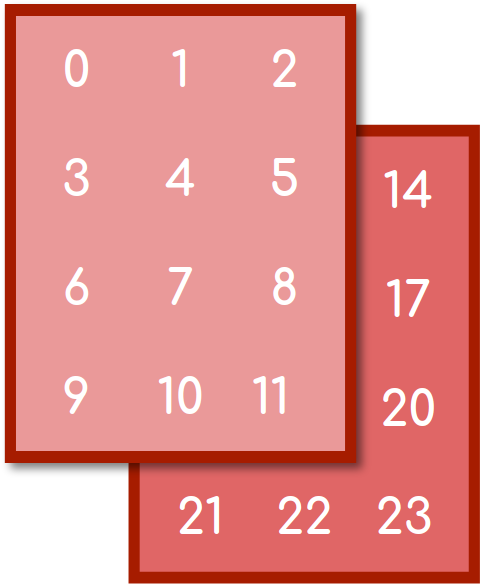
\includegraphics[height=10em]{tensors/order3}
		\caption{Order-3 tensor}
	\end{subfigure}
	\caption[Depictions of tensors of various orders]{Depictions of tensors of various orders.}
	\label{fig:tensor_orders}
\end{figure}

A tensor's shape refers to its size in each of its dimensions; so the tensors in Figure~\ref{fig:tensor_orders} are of shapes $(3)
$, $(4,3)$ and $(2,4,3)$, respectively. Tensor operations manipulate these tensors, performing linear algebra transformations
over their contents. While the normal set of linear algebra operations like additions and inner products are used fairly commonly in neural networks, there are more domain-specific and specialized ones that are also very common.

\subsection{Nonlinearities}~\label{sect:nonlinearities}
The simplest form of tensor operation is the nonlinearity or activation function, a nonlinear function that often
maps $\mathbb{R}$ into some subset of $\mathbb{R}$. These nonlinearities allow for more complex functions to be modelled,
thus turning the purely linear combinations produced by neurons into Universal Approximators~\citep{stinchcombe1989}.

\begin{figure}[ht]
	\centering
	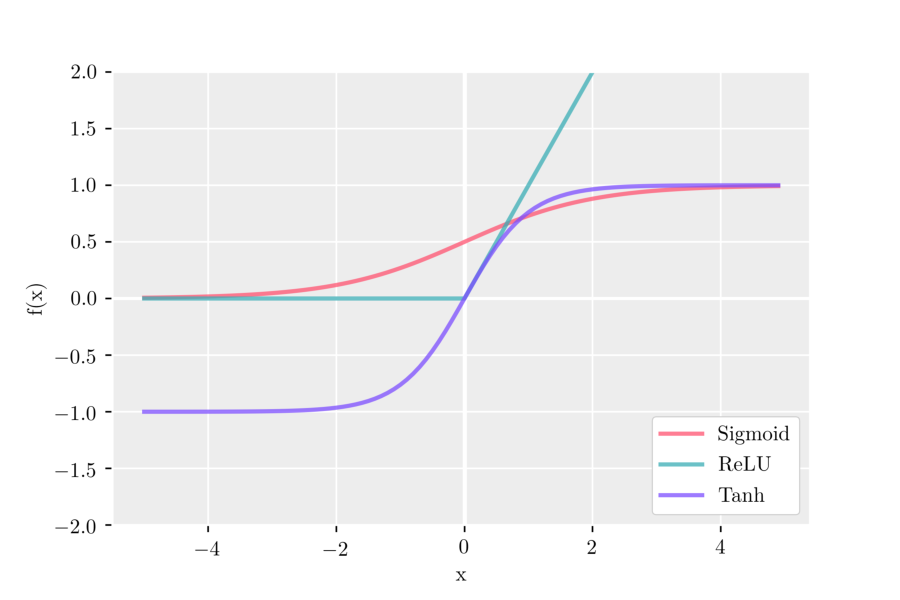
\includegraphics[width=\textwidth]{tensors/ops/nonlins.pdf}
	\caption[The three most common tensor nonlinearties]{The three most common tensor nonlinearities.}
	\label{fig:nonlins}
\end{figure}
\begin{align}
	\text{Sigmoid}(x) \quad &= \quad\frac{1}{1+e^{-x}} \label{eq:sig} &\\[5pt]
	\text{ReLU}(x)\quad &= \quad\begin{cases}
									x ,& x>0 \\
									0 ,& x\le0
	\end{cases} \label{eq:relu}&\\[4pt]
	\text{Tanh(x)} \quad &= \quad \frac{e^x - e^{-x}}{e^x + e^{-x}} \label{eq:tanh}
\end{align}
The three most common types of nonlinearity used are the sigmoid (Equation~\ref{eq:sig}), the rectified linear unit (ReLU, Equation~\ref{eq:relu}),
or the hyperbolic tangent (tanh, Equation~\ref{eq:tanh}).
Sigmoids and tanhs are closely mathematically related and often serve similar purposes within neural nets, and their ability to
map $ \mathbb{R}$ into a very restricted space serves well to prevent a neural net phenomenon called gradient explosion.
Gradient explosion can occur during network training, where the learnable weights of the network are updated proportionally
to their error gradient (more on this later). In cases where this error gradient is very large, it can create a positive
feedback loop, and rapidly send the weights and outputs of a function to positive or negative infinity. With the tanh and sigmoid,
this is prevented because $|f(x)|\ll|x|$ for the majority of $x$ values, which clamps down the feedback loop and ensures
that this runaway effect never occurs.

However, this exact behavior causes another issue to arise, and that is the dying gradient problem.
In cases where the sigmoid and tanh function are receiving values of such that $|x|\gg0$ (called saturation),
the derivatives of these nonlinearities with respect to these
extreme inputs are zero. This in turn means the error gradient and thus the proportional weight update are also zero, meaning the
network cannot update the neuron weights and the neuron is stuck at this saturated value.
This causes poor model training results, and tends to limit the depth of networks that make use of sigmoid or
tanh activations~\citep{maas2013}.

ReLUs seek to remedy this issue by eliminating positive saturation, allowing positive values to flow unaltered through the activation.
This is more biologically similar to organic neurons which exhibit the same thresholding behavior as the ReLU, which is
where the ReLU equation draws inspiration~\citep{glorot2011}.
While~\citeauthor{glorot2011} note that negative saturation is hard-coded into ReLUs and is more extreme than in either sigmoid or
tanh activations (i.e., the gradient for all $x<0$ is always 0), the original authors note that it does not have
particularly adverse effects on model training performance.
They theorize that this is due to the counter-balancing effects of other parallel unsaturated neurons, which are
more prevalent in ReLU networks due to their single direction of saturation.
However, since ReLUs do not throttle positive inputs, gradient explosion can be a significant problem. Despite this, ReLUs
are typically the activation of choice in modern models, helped by their relatively minimal computational cost compared to
others.

\subsection{Batch Normalization} \label{sect:batch_norm}
To remedy both dying and exploding gradients,~\cite{ioffe2015} introduced batch normalization.
Batch normalization simply ensures that each batch of tensors
that pass through the operation are first normalized to mean 0 and variance 1, before a learned scaling $\gamma$ and shifting $\beta$ is applied:
\begin{align}
	\hat{x_i} &= \frac{x_i - \mu_{\mathit{B}}}{\sqrt{\sigma^2_\mathit{B} + \epsilon}} & \text{(Normalize according to batch mean } \mu_{\mathit{B}} \text{ and variance } \sigma^2_\mathit{B}) &\\
	y_i &= \gamma \hat{x_i} + \beta  &(\text{Scale by } \gamma \text{ and shift by } \beta\text{, values set by network's particular needs})
\end{align}
The mean and variance are computed per-batch during training, while the running averages of these statistics are
used to estimate the population mean and variance during inference. Performing this normalization on a per-batch basis
as opposed to globally is more computationally efficient and allows for the influence of the normalization to be
differentiable, meaning that it can be seamlessly incorporated into backpropagation without modification. The second step
of the batch-normalization function, the scale and shift, is in place so that the original
`intent' of the operation can be maintained; consider a sigmoid operation to understand why this is necessary.
Around zero, it is more or less a linear mapping. In large positive or negative regions, it is a hard mapping to 1 or -1.
Were all inputs to a sigmoid function normalized to mean 0 and variance 1, the sigmoid is rendered mostly useless. As such,
the output of the batch-normalization can be shifted or scaled such that the model can align it with the desired input
distribution of the subsequent operation.

Allowing the model to set a desired region in which each input distribution should lie in mitigates a crucial issue
known as covariate shift. This occurs when the distributions of input to some learned function changes over the
course of training. Imagine some deep layer $f_n$ of the network, whose input $x_n$ is some combination and
composition of all the previous operations in the network:
\begin{align}
	x_n = f_{n-1}\left( f_{n-2} \left( f_{n-3} \left( \dots f_{1} \left(x_1\right) \right) \right) \right)
\end{align}
\overfullrule=0pt
As the network learns, the output distributions of each of the layer operations $f_{n-1}, f_{n-2}, \dots , f_1$ will change. This is a compounding effect, in that each change to the output distribution of an early layer will effect the input distributions
of later layers, thus influencing their output distributions in turn, and so on. This means that these later layers will have to keep adapting their parameters for these changing inputs, having to accommodate constant fluctuations in input distribution.
By enforcing a consistent distribution that will always lie in some desired location, batch normalization allows operations
to spend the entire training process specializing to their specific task in the network, and should therefore converge must
faster than operations that had to constantly adjust for changing input distributions. Ioffe and Szegedy found this to be
exactly the case; models with batch-normalization operations converged around five times faster than models without.

\subsection{Convolutions}  \label{sect:conv}
When working with higher dimensional input data such as images, it can get very computationally expensive to use pure
feedforward networks. For a very small input 32x32 image with three color dimensions, the corresponding tensor has a shape of
(3, 32, 32): a 3072 dimensional input to the model. Simply adding a single feedforward layer of comparable dimension requires on the order of 10 million
differentiable parameters. Furthermore, there is a structural facet to the input data; in images,
information is likely to be highly locally correlated both spatially and colorwise. This means the
properties of regions are likely to be more interesting than individual points, and want to perform operations that can meaningfully extract this spatial
information: learning how these local regions interact is more useful than
the relation between remote regions. While feedforward layers could in theory learn this spatial dependence, it would require a lot of
serendipitous coordination.  Each neuron in a fully-connected layer receives input from all previous neurons,
so a neuron trying to focus locally would need to set a majority of its input weights to 0 to achieve this behavior.
Another consideration when working with images is translational invariance; under many circumstances,
the ground-truth function $f'(x)$ of an image does not change if the contents of the image change their position.
For example, if the ground-truth function is to identify the animal within an image, an image of a dog is still an image
of a dog regardless of where it appears within the borders of the image.

While fully-connected layers could in theory
learn all of these desirable behaviors given enough time and favorable training material, it makes a lot more sense
to directly use an operation that comes with all of them built in, and this operation is the convolution.
Tensor convolutions are operations that filter some n-dimensional input tensor $\mathbf{A}$ by some kernel $\mathbf{K}$:
\begin{align}
	(\mathbf{A} ** \mathbf{K})_{x_1,\dots,x_n} = \sum_{i_1\in\mathbb{Z}}\dots\sum_{i_n\in\mathbb{Z}} \mathbf{K}(i_1,\dots,i_n)\mathbf{A}(x_1-i_1,\dots,x_n-i_n)
\end{align}
\noindent This equation slides the kernel $\mathbf{K}$ over every element of the input signal $\mathbf{A}$.
At each position, it takes the Frobenius inner product\footnote{The Frobenius inner product is an adaptation of the vector
dot product tailored for use with matrices; it is computed as the sum of the element-wise product of two matrices:
	$\left<\mathbf{A},\mathbf{B}\right>_F = \sum_i \sum_j \mathbf{A}_{ij} \mathbf{B}_{ij}$}  of the kernel and the
overlapped region of the input.

In practice, these convolutions are almost exclusively used in two-dimensional cases wherein $\mathbf{K}$ is only defined over some finite range $[-m,m]$
and $\mathbf{A}$ over some range $[-n,n]$. Outside the range $[-n,n]$, the signal is `zero-padded' setting $A(x_1,x_2,\ldots,x_n) = 0$
if any $x_i$ is outside the range $[-m,m]$, which serves in the case wherein $\mathbf{A}$ is indexed in an undefined region. In this two-dimensional, finite case,
the equation becomes:
\begin{align}
	(\mathbf{A} ** \mathbf{K})_{x_1,x_2} = \sum_{i_1=-m}^{m}\sum_{i_2=-m}^{m} \mathbf{K}(i_1,i_2)\mathbf{A}(x_1-i_1,x_2-i_2)
\end{align}

 For example:
\begin{alignat}{3}
	\text{If}\; \mathbf{A} &= \ilmat{10}{A.png} \quad && \text{and} \quad &&\mathbf{K}= \ilmat{10}{K.png} \; \text{, then:}
\end{alignat}
\vspace{-1.2em}
\begin{alignat}{3}
	(\mathbf{A}** \mathbf{K})_{1,1} &= \ilmat{13}{A_K_11.png} &&= \left<\ilmat{10}{K.png}\botcomma \ilmat{10}{A_sub1.png}\right>_F &&= 4 \\
	(\mathbf{A}** \mathbf{K})_{1,2} &= \ilmat{13}{A_K_12.png} &&= \left<\ilmat{10}{K.png}\botcomma \ilmat{10}{A_sub2.png}\right>_F &&= 6 \\
	(\mathbf{A}** \mathbf{K})_{1,3} &= \ilmat{13}{A_K_13.png} &&= \left<\ilmat{10}{K.png}\botcomma \ilmat{10}{A_sub3.png}\right>_F &&= 6
\end{alignat}
and so on, such that the final output is:

\begin{align}
	\mathbf{A}** \mathbf{K} = \ilmat{10}{A_K.png}
\end{align}

These kernels filter the input data, and as such can highlight or suppress certain features of the data
depending on the contents of the kernel. Working with some examples will demonstrate how this can be useful. Since
the predominant use case for these convolutional kernels in the field is for image processing, images will be used as
input data in these examples. A color image can be thought of as a stack of three two-dimensional matrices, one matrix (or channel) for
the red values at each point, one for blue, and one for green. Then, the kernel will be applied to each channel of the image
(essentially performing three separate convolutions) and then the final output will demonstrate what the kernel has
extracted or suppressed. Figure~\ref{fig:convolutions} looks at two $3\times 3$ kernels, and shows the results produced by
convolving images with these kernels:

\newcommand{\kblur}{\mathbf{K}_{blur} = \ilmat{10}{K_blur}}
\newcommand{\kvert}{\mathbf{K}_{edge} = \ilmat{10}{K_vert}}
\newcommand{\imgconv}[1]{\vcenter{\hbox{\includegraphics[width=.8\textwidth]{convs/#1}}}}


\begin{figure}[ht!]
	\centering
	\begin{subfigure}[b]{0.32\textwidth}
		\centering
		\makebox[\textwidth]{\textbf{Original Images:}}
	\end{subfigure}
	\begin{subfigure}[b]{0.32\textwidth}
		\centering
		$\imgconv{boat_orig}$
	\end{subfigure}
	\begin{subfigure}[b]{0.32\textwidth}
		\centering
		$\imgconv{bus_orig}$
	\end{subfigure}
	\rule{\textwidth}{1pt}
	\par\bigskip
	\begin{subfigure}[b]{0.32\textwidth}
		\centering
		$\kblur$
	\end{subfigure}
	\begin{subfigure}[b]{0.32\textwidth}
		\centering
		$\imgconv{boat_blur}$
	\end{subfigure}
	\begin{subfigure}[b]{0.32\textwidth}
		\centering
		$\imgconv{bus_blur}$
	\end{subfigure}
	\caption{Blurring kernel}
	\rule{\textwidth}{1pt}
	\par\bigskip
	\begin{subfigure}[b]{0.32\textwidth}
		\centering
		$\kvert$
	\end{subfigure}
	\begin{subfigure}[b]{0.32\textwidth}
		\centering
		$\imgconv{boat_edge}$
	\end{subfigure}
	\begin{subfigure}[b]{0.32\textwidth}
		\centering
		$\imgconv{bus_edge}$
	\end{subfigure}
	\label{fig:convolutions}
	\caption{Edge detection kernel}
\end{figure}

The first kernel $\mathbf{K}_{blur}$ will return a weighted sum of each of the nine points overlapped by the kernel;
this is equivalent to the average pixel value of the nine points. The end effect of this is that each pixel in the
output image is the average value of the 3x3 region centered at that point in the input image, producing a blurring effect.

The second kernel $\mathbf{K}_{edge}$ extracts edges in the input image. This is because in regions with uniform
color information (and thus edgeless regions), the strongly weighted center point will get counterbalanced by the
negatively weighted outer points. The only way for this to return nonzero is if some of the outer points have
strongly different information than the center point, which would occur at color boundaries. This therefore means the
output image is nonzero only along such boundaries, thus extracting edges.

While these two kernels are hand-designed to work specifically for images (and to produce good looking results for
this example), convolutional layers within models can discover and learn kernels that best extract relevant
information from the data passing through their particular layer within the network. There are a few different
types of the convolutional layers, which all serve different purposes within models. The most common type
applies multi-dimensional kernels of shape $(N,M,k_1,..,k_n)$, where $N$ refers to the number of output channels, $M$
the number of input channels, and $k_1,\dots,k_n$ to the size of the kernel in each spatial dimension. The
kernels given above in Figure~\ref{fig:convolutions} would be of shape $(3,3,3,3)$, as they were each $3 \times 3$ kernels that received and
outputted the three color channels in the image. The general equation for this class of convolutional layers is:

\begin{align}
	\mathbf{C}^{out}_{n} = \sum_{m=1}^{M} (\mathbf{C}^{in}_{m} ** \mathbf{K}_{nm})  \label{eq:conv}
\end{align}
Here, $\mathbf{K}_{nm}$ refers to the $(N,M,k_1,..,k_n)$ kernel tensor sliced at the $n$th output dimension and $m$th input dimension.
For example, if there are four input channels and two output channels are desired, the kernel tensor would be
of shape $(2,4,k_1,..,k_n)$, and the first output channel would be calculated as follows:
\begin{align}
	\mathbf{C}^{out}_1 &=  \sum_{m=1}^{4} (\mathbf{C}^{in}_{m} **  \mathbf{K}_{1m}) \\
	\mathbf{C}^{out}_1 &=  \sum \left(\quad \vcenter{\hbox{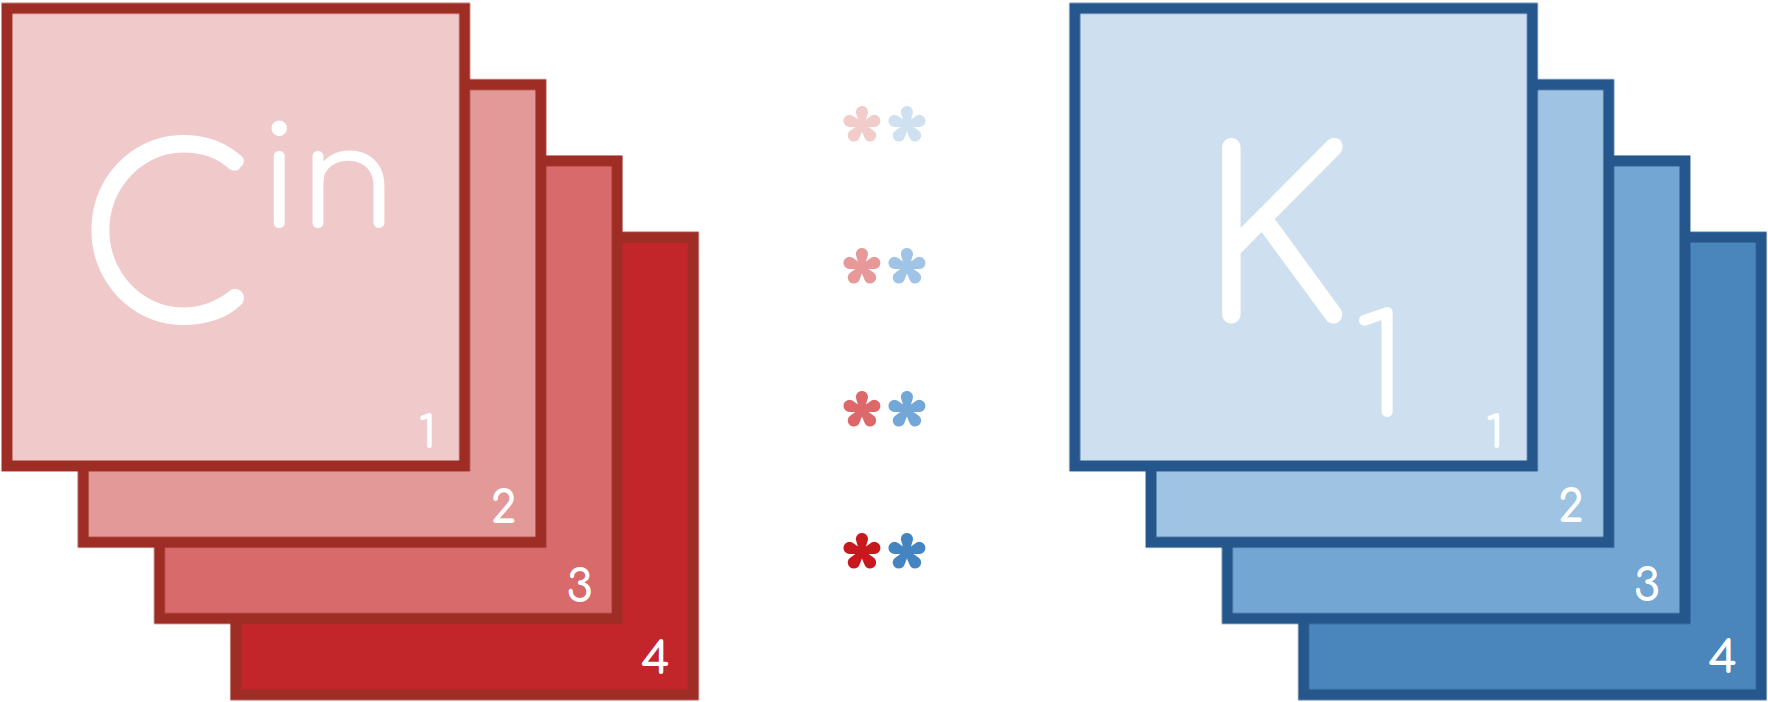
\includegraphics[height=22ex]{convs/chan_stack}}}\quad \right) \\[1em]
\end{align}
\noindent and the second output channel:
\begin{align}
	\mathbf{C}^{out}_2 &=  \sum_{m=1}^{4} (\mathbf{C}^{in}_{m} **  \mathbf{K}_{2m}) \\
	\mathbf{C}^{out}_2 &=  \sum \left(\quad \vcenter{\hbox{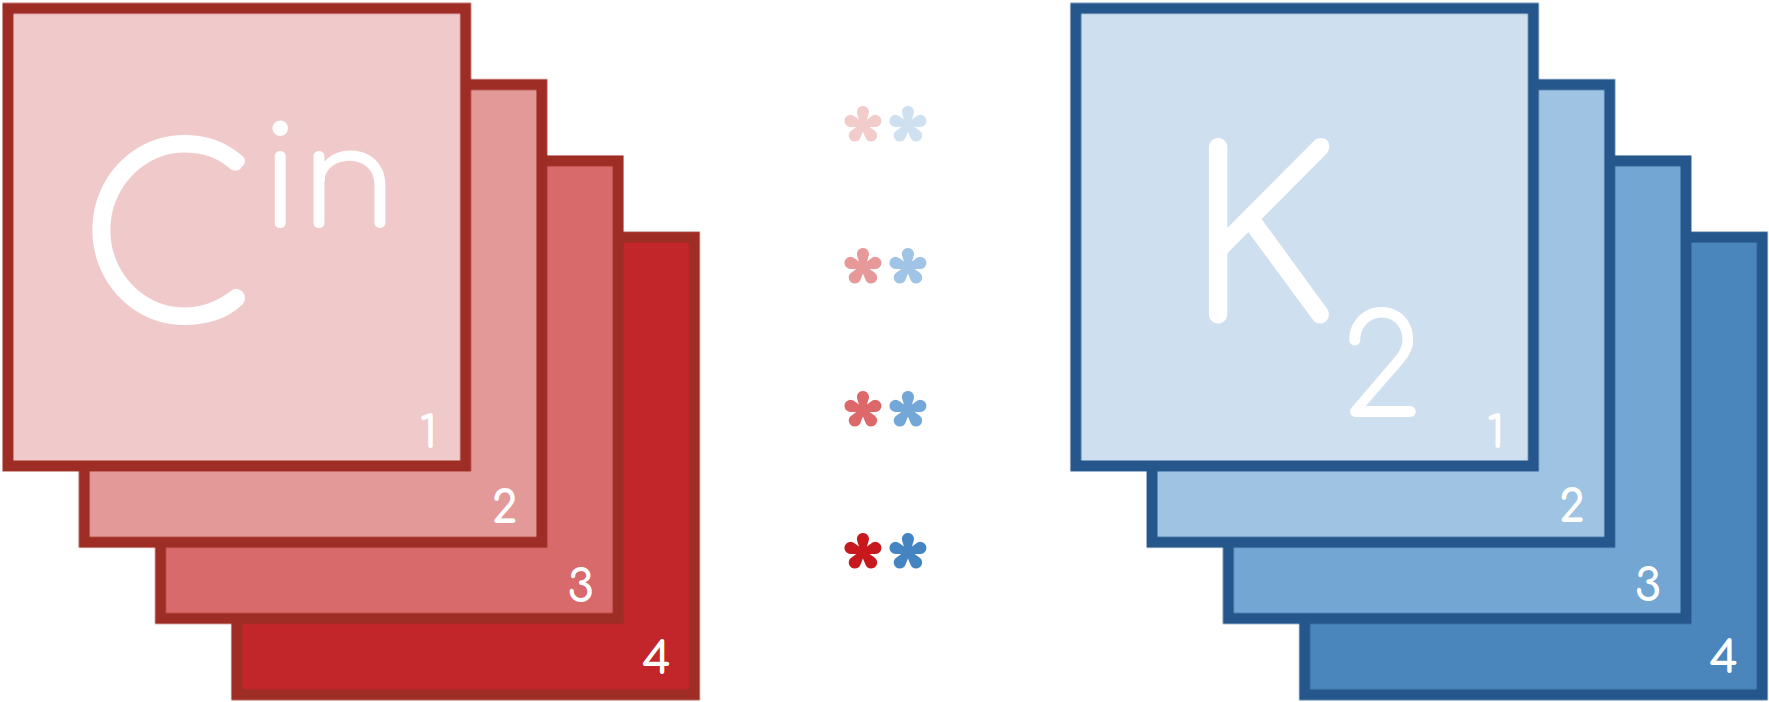
\includegraphics[height=22ex]{convs/chan_stack2}}}\quad \right)
\end{align}

A subtype of this vanilla $k\times k$ convolution is the $1\times1$ convolution or the Network-in-Network, introduced
in a 2013 paper of the same name~\citep{lin2013}. These convolutions involve $1\times1$ convolutional kernels,
which means the convolutional equation simplifies to:

\begin{align}
	 \mathbf{C}^{out}_n  &= (\mathbf{A} ** \mathbf{K})_{x_1,x_2} \\
	 &= k\mathbf{A}(x_1,x_2) \\
	 &= \sum_{m=1}^4 (k_{n,m}\mathbf{C}^{in}_m)
\end{align}
\noindent where $k_{n,m}$ is the single value that arises when the $n$th $1\times1$ kernel $\mathbf{K}_n$ is sliced along channel dimension $m$. In essence, this means that each $1\times1$ convolutional kernel is performing a weighted sum of the values of the input channel. The output is thus $N$ weighted sums of the input, meaning the 1x1 convolution is the equivalent of a $M$-$N$ fully connected layer, hence the name Network-in-Network.

\subsection{Poolings}
While convolutions are an excellent means of efficiently extracting information about local patterns within a tensor,
they are still relatively expensive to train; a $k_1*k_2$ convolutional kernel with $N$ input channels and $M$ output channels
has $k_1*k_2*N*M$ parameters to learn. In circumstances where it is more important to aggregate local patterns than
synthesise new information about these patterns, some interesting kernels can be `pre-baked' to perform these aggregations
with no need for training. Such aggregations are called \textit{pooling} operations, and they simply aggregate local
information in some preset way. The two most common pooling operations in literature are by far Max Pooling and
Average Pooling. The former is a kernel that simply returns the max value found within the kernel, while the
latter operates identically to the blurring kernel discussed in Figure~\ref{fig:convolutions}, returning the mean value
of the values within the kernel.

\begin{align}
	\text{Max Pool}_{3x3}\left( \; \ilmat{10}{A.png} \; \right) &= \max(0,1,2,3,4,5,6,7,8) = 8 &\\
	\text{Average Pool}_{3x3}\left( \; \ilmat{10}{A.png} \; \right) &= \text{mean}(0,1,2,3,4,5,6,7,8) = 4
\end{align}

Commonly, pooling operations are used to downsample images, that is, shrink them down to some smaller height and width.
This is done by changing the operation's \textit{stride} $s$ to some value greater than 1. Stride sets the step size of the kernel as it slides
over the input image, which has the effect of sampling the result of the pooling operation at every $s$th
location. This in turn reduces the output size of the operation by a factor of $s$. For example, a stride=2 pooling applied to a
$50 \times 50$ pixel image would produce a $25 \times 25$ output.

\section{Convolutional Neural Networks} \label{sect:nn_advanced_end}
By taking the operations described above and combining them in various connectivity patterns, models can be designed that
can take advantage of the variety of desirable mathematics that these operations hold. These models are
referred to as \textit{Convolutional Neural Networks} or CNNs. Typically, the convolutional neural network gets its name
from the operation that most commonly makes up the majority of its internal transformations, but there is nothing preventing
a CNN from having a majority of pooling operations or non-linearities.

\section{Datasets} \label{sect:data_policies}
The two most important things that shape the design of deep learning models are the data and task to which the model is intended
to be applied. The data heavily affect the internal mathematics of the model, that is, determining which kind of tensor
operations are most applicable to this domain of data. Image data, for example, are often paired with
convolutional operations because they are capable of providing significant performance very efficiently. Meanwhile,
the task the model is intended to perform also affects the model connectivity and the architecture, particularly the structure
of the later stages and output of the model. Due to this co-mingling influence of data and task, it is helpful to wrap them
together into a single conceptual unit. Henceforth, a deep-learning `problem' refers to this conceptual unit, the joint data
and task pair that is being worked with.

However, while building models for a specific, individualized problem is useful to those individuals grappling with said problem,
it may be of limited applicability in other domains. As such, in order to create truly generalizable approaches that are
appropriate for a wide variety of applications, it is imperative to work with problems that are proxies for an entire domain of problems.
The ideal proxy problem is one that is truly generalizable, wherein a model that performs well on the proxy will
perform well in any problem within the proxied domain. These proxy problems come to represent the entire data domain,
where showing performance on one of these proxy problems is a shorthand for claiming equal performance on any such problem.

\subsection{MNIST}
\begin{figure}[htbp!]
\centering
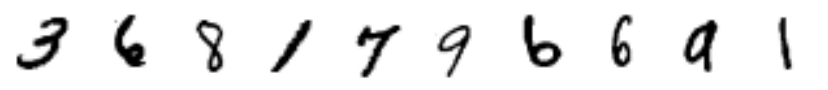
\includegraphics[width=1\textwidth]{data/mnist_sample}
\caption[Sample MNIST images]{Some sample images from the MNIST dataset, as presented in the original 1998 paper.}
\label{fig:mnist}
\end{figure}

One the earliest such sets of proxy problems for visual classification was the MNIST handwritten digit classification problem,
introduced in~\cite{lecun1998}. This dataset is based
on two datasets of binary images of handwritten digits published by the American National Institute of Standards and Technology,
(NIST) one taken from a sample of census workers and the other high school students. Each image of a handwritten digit
was paired with its corresponding label from 0 to 9, meaning it is a 10 class classification problem.
\citeauthor{lecun1998} combined the two datasets into a distinct train and test set, such that both types of writer appeared in both
sets but no individual writer overlapped the two sets. This left them with 60,000 training images and 10,000 test images,
each 28x28 pixels in size. 10 such images are shown in Figure~\ref{fig:mnist}. They dubbed this dataset the Modified NIST dataset, or MNIST for short, and provided some
examples of convolutional neural network performance over this dataset. While the largest feasible convolutional
neural networks in 1998 are orders of magnitude smaller than the ones used today, their networks managed to achieve up
to 99.3\% accuracy on the test set.

MNIST is a very small dataset, due to both being monochromatic and having a compact image size, and has well-distinguished
classes. While these attributes make it very portable and quick to work with, it means the task is relatively simple.
This is evidenced by the remarkable performance \citeauthor{lecun1998} managed to find with the rudimentary networks of 1998. This
fact has caused MNIST to fall out of prominence as a computer vision proxy problem; there is very little to prove in scoring
very highly on MNIST. If a 99.3\% was possible in 1998, it is not particularly impressive to do better in 2021.


\subsection{CIFAR}
\begin{figure}[htbp!]
\centering
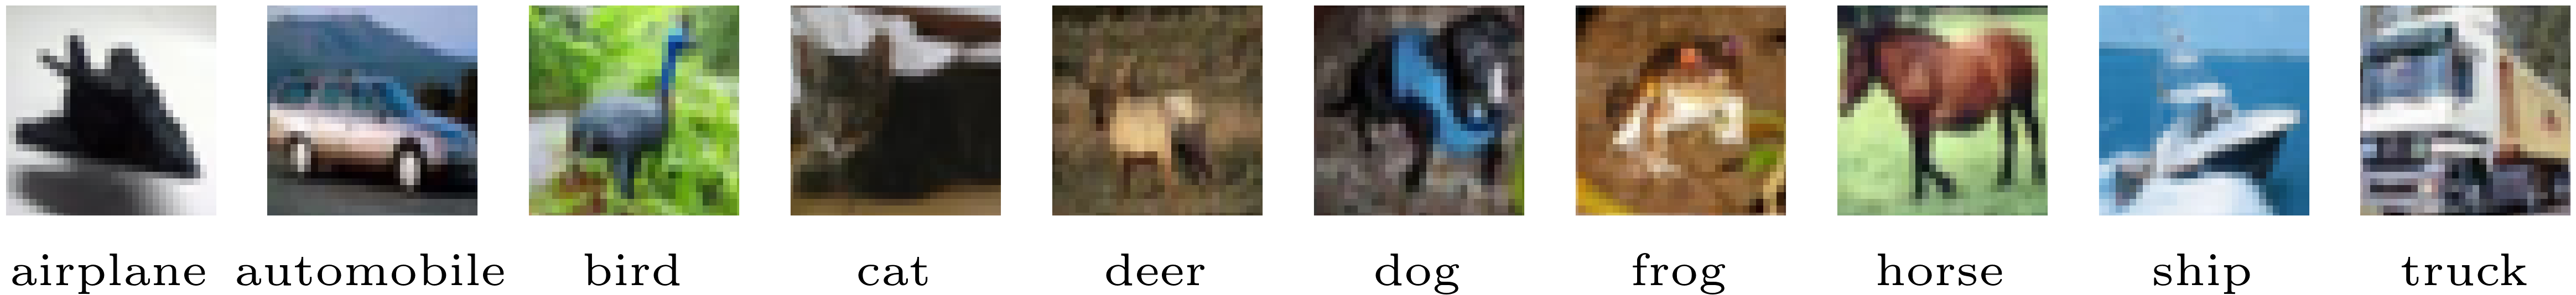
\includegraphics[width=1\textwidth]{data/cifar10_sample}
\caption[Sample CIFAR-10 images]{An image from each class of the CIFAR-10 dataset.}
\label{fig:cifar10}
\end{figure}

In the name of introducing a dataset involving ``real'', full color images,~\cite{kriv2009} introduced the CIFAR family
of classification problems. Krizhevsky argued that full color, real images, that is, ones that are actual
photos of real world objects, demonstrate unique data correlations. Specifically, pixels are strongly correlated to nearby
pixels and weakly correlated to distant ones, and same-channel correlations between neighboring pixels are much
stronger than cross-channel correlations. Furthermore, Krizhevsky comments on the lack of useful labels on existing datasets,
specifically referring to the MIT Tiny Images dataset~\citep{torralba2008}.

To address this, a 60,000 image subset of the Tiny Images dataset was hand-labelled into 10 classes, and another 60,000
image subset into 100 classes. Each image is 3\texttimes32\texttimes32, with the first dimension representing the three color channels of
the RGB image. These two subsets were named the CIFAR-10 and CIFAR-100 datasets, after the Canadian Institute For Advanced
Research. Ten CIFAR-10 images are shown in Figure~\ref{fig:cifar10}, one from each class. Of the two datasets,
CIFAR-10 is by far the most popular, due to its conciseness; it is easy to visually distinguish, remember,
and program the 10 available classes as compared to the more numerous and nuanced classes of CIFAR-100.

As a result, CIFAR-10 is ubiquitous within the field of computer vision, with the original paper having around 10,000
citations on Google Scholar and the search term ``CIFAR-10'' yielding 360,000 Google search results as of March 2021,
and as such is one of the most common benchmarks researchers use to compare their models against competitors. As
of March 2021, state-of-the-art results on CIFAR-10 tend to range from 97\% to 99\% classification accuracy, with the
record score of 99.0\% being held by GPipe~\citep{huang2018}. While accuracy is generally the most common and considered
metric for CIFAR models, parameter count serves as an additional orthogonal direction of research. Both directions have
been explored in recent papers, with papers like DARTS~\citep{liu2018} highlighting their technique's relatively low 3.3
million parameters as more portable and compact than the competition, while GPipe's ability to scale up to a massive 83.9
billion parameters is promoted as unprecedented and unparalleled. Both directions are important, in that compactness
and portability are tremendously useful in bringing the power of deep learning to a wider range of devices, while sheer
size is often the key to unlocking higher model performance~\citep{tan2019}.

\subsection{ImageNet}
\begin{figure}[htbp!]
\centering
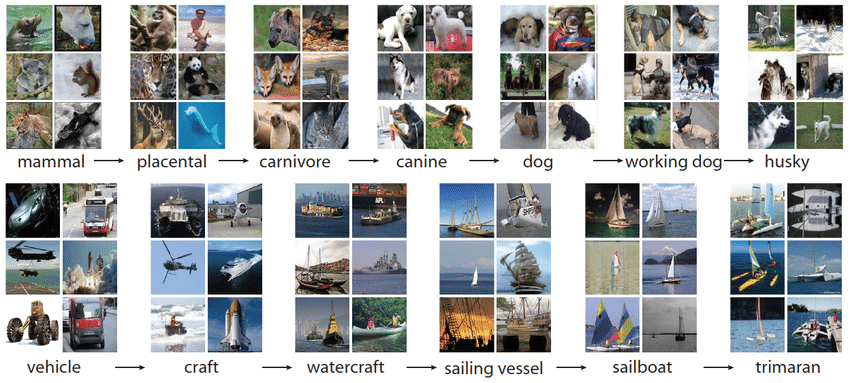
\includegraphics[width=1\textwidth]{data/imagenet_sample}
\caption[Sample ImageNet images]{Some sample images within the ImageNet dataset~\citep{ye2018}.}
\label{fig:imagenet}
\end{figure}
While CIFAR-10's appeal lies in its simplicity and comprehensibility at the expense of broad generalizability, ImageNet's
appeal is the exact opposite.
The ImageNet dataset~\citep{deng2009,deng2014} is a collection of 3.2 million images, released in 2009 and based on the
WordNet semantic hierarchy. This semantic hierarchy organizes words into a tree, wherein each word in the tree could also
be meaningfully described by every word in its antecedent nodes. For example, the traversal to the word `computer' is:

\begin{center}
\texttt{artifact} $\rightarrow$ \texttt{instrument} $\rightarrow$ \texttt{device} $\rightarrow$ \texttt{machine} $\rightarrow$ \texttt{computer}
\end{center}

\noindent while the traversal to the word `skateboard' is:
\begin{center}
\texttt{artifact} $\rightarrow$ \texttt{instrument} $\rightarrow$ \texttt{conveyance} $\rightarrow$ \texttt{vehicle} $\rightarrow$ \texttt{wheeled vehicle} $\rightarrow$ \texttt{skateboard}
\end{center}

\noindent
\added{For more more traversals with accompanying images, see Figure~\ref{fig:imagenet}.}
The images within the ImageNet data are labelled in this manner, which means the label of each image conveys not only
the contents of the image but its place within the overarching semantic tree as well. There are 21,841 distinct labels,
and as such ImageNet contains an extraordinary catalogue of objects by which to evaluate the capabilities of a computer
vision model. Models trained on the entire 14 million image ImageNet dataset would generalize extraordinarily well to
other image classification problems due to its implicit comprehensiveness; the model has likely already seen whatever
it is that the new problem would ask it to classify.

There is a variety of tasks based upon this dataset, but the most common one in the particular field of deep learning
architecture research is the aforementioned ImageNet Large Scale Visual Recognition Challenge or ILSVRC, specifically
the image classification challenge. This consists of a non-overlapping subset of 1000 classes within the full ImageNet
data, with around 1000 images per class, for a total data size of 1,281,167 images. The objective is to classify these
images, and often both top-1 and top-5 accuracy are given due to the subtler nature of the class distinctions. The record
for this problem is 84.3\% top-1 and 97\% top-5 accuracy, also held by GPipe. Again, parameter count is recorded as well,
with ongoing research into pushing the boundaries in both directions.

\section{Software and Hardware} \label{sect:hardware}
With the basic theoretical concepts of deep learning outlined, the practical aspects necessary to
perform it can be explored.

\subsection{GPUs and CUDA}
The predominant means of performing deep learning at scale is through the use of Graphics Processing
Units (GPUs). A GPU is designed to perform massively parallel linear algebra computation for the purposes
of digital rendering, however, these exact computations can be leveraged to rapidly acceralate deep learning~\citep{kriv2012}
as compared to a purely CPU-based computation system.
CUDA (Compute Unified Device Architecture) is a parallel computation library released in 2006 by~\citeauthor{CUDASite},
specifically designed to make the compute capabilities of modern GPUs accessible to user programs. For the purposes of this thesis, CUDA serves
as a means of performing very large linear algebra operations very rapidly,
such as those used ubiquitously throughout neural networks such as Equation~\ref{eq:ffw_layer} or~\ref{eq:conv}.

The main limitation to the scale of these operations comes in the form of the GPU's video memory, or VRAM.
The inputs, outputs, and intermediate
values of any calculation performed on the GPU must be stored in VRAM, which places a limit on the possible
parallelization and input size of any calculation. Modern, commercially-available GPUs have on the order of
8 GB to 24 GB of VRAM, which corresponds to between 2 and 6 billion 32-bit floats at maximum that can be allocated at once.
While this seems massive, a normal batch of image inputs to a convolutional neural network can have on the order of
200,000 floats, which means there is only space to perform around 10,000-30,000 manipulations of this input.
Considering that some neural networks can have upwards of 100 million differentiable parameters, each of which could potentially
require a full allocation of another 200,000 floats, the available VRAM space can be consumed very quickly. Management
of the available VRAM space is one of the chief design considerations of neural networks, such as to ensure that this
space is used as efficiently and effectively as possible.

\subsection{Torch}
The most common way to use CUDA operations is to use a library that interfaces with them, at least in the field of
machine learning. This allows easy access to the benefits of CUDA's parallelization ability without the need to work
directly with CUDA's GPU APIs in C. The significant majority of published deep learning papers that release their codebases
are written in Python, and the most common Python libraries for interfacing with CUDA are PyTorch~\citep{paszke2019}
and TensorFlow~\citep{abadi2016}. While for the most part the two are very similar in capability, PyTorch's
organizational style is particularly clear and elegant, particularly its highly object-oriented approach to model construction.
As such, the entirety of the deep learning work in this thesis is written in Python and heavily utilizes PyTorch.

At its core, PyTorch is a tensor processing library that uses CUDA operations to drastically speed
up computation time. It also provides a library named \texttt{torch.nn}, which builds a neural network construction framework
on top of the tensor functionality. PyTorch structures neural models as computation graphs, and provides inference
and back-propagation functionality through traversals of this graph. Model inference involves traversing this graph
from input to output, and is called the \texttt{forward} function of the model. Backpropagation traverses the graph in the
opposite direction, automatically computing the gradients of each parameter with respect to the output loss
along the way via the chain rule. The backwards pass is
aptly named the \texttt{backward} function of the model. The primary advantage of using such a library is automatic
computation of these partial gradients for a suite of operations that come bundled into the library, which allows
users the flexibility of combining multiple components together into new and interesting compositions without worrying
about computing their derivational properties.

When writing these compositions, an important thing to be cognizant of is the function trace of the various PyTorch
operations being used. Each function within PyTorch is often comprised of a variety of underlying C or CUDA functions,
the complexities and number of which vary depending on the mathematical properties of the operation and whether the operation
is being run in the forwards or backwards direction. Some operations are deceptive in this regards, with things
like tensor indexing (accessing the $n$th item of a tensor) being very quick and efficient in the forwards direction,
but painfully slow and expensive in the backwards direction. This means that code optimization in PyTorch takes on a
new and unfamiliar dimension; optimizations must be effective in both the forward pass and in the often less tractable
gradient calculations within the backwards pass.

One final idiosyncrasy to note is the problem of stuck tensors in the case of VRAM out-of-memory errors. PyTorch
automatically and intelligently clears tensors out of VRAM when they are no longer in use, dynamically freeing memory
to be reallocated later. However, this intelligent garbage collection breaks down when tensor allocation fails due to
insufficient available VRAM; this failure can cause all tensors that currently exist on the GPU to become stuck there,
unable to be freed unless the entire Python kernel that originally allocated them is killed. This can be disastrous in
cases where these out-of-memory errors crop up late in model training, as this means the model and its weights
must be deleted in order to clear the stuck tensors.

\section{Conclusion}
This chapter consitutes the necessary foundations of deep learning and computer vision to understand this work. For
more information on what has been covered thus far,~\cite{goodfellow2016}
is an excellent reference textbook. Now, the specific world of state-of-the-art computer vision models can be explored,
as can the neural architecture search techniques that
strive to automatically generate them.